\documentclass[10pt,a4paper,onecolumn]{article}
\usepackage{marginnote}
\usepackage{graphicx}
%\usepackage{xcolor}
\usepackage[dvipsnames]{xcolor}
\usepackage{authblk,etoolbox}
\usepackage{titlesec}
\usepackage{calc}
\usepackage{tikz}
% use microtype if available
\IfFileExists{microtype.sty}{%
\usepackage{microtype}
\UseMicrotypeSet[protrusion]{basicmath} % disable protrusion for tt fonts
}{}
\usepackage{setspace}
\usepackage{hyperref}
\hypersetup{colorlinks,
            urlcolor=NavyBlue,
            linkcolor=Mulberry}
\usepackage{caption}
\usepackage{tcolorbox}
\usepackage{amssymb,amsmath}
\usepackage{ifxetex,ifluatex}
\usepackage{seqsplit}
\usepackage{enumitem}
\usepackage{xparse}

\usepackage{balance}

\ExplSyntaxOn

\clist_new:N \g_mapo_allauthors_clist

\NewDocumentCommand\addauthor {m}
 {
  \clist_gput_right:Nn \g_mapo_allauthors_clist { #1 }
 }

\NewDocumentCommand \printall { } { } % initialization
\DeclareExpandableDocumentCommand \printall { }
 {
  \clist_use:Nnnn \g_mapo_allauthors_clist { ~and~ } { ,~ } { ~and~ }
 }

\ExplSyntaxOff

% \usepackage{fixltx2e} % provides \textsubscript
\usepackage[backend=biber,style=apa]{biblatex}

\addbibresource{master.bib}
\addbibresource{packages.bib}

% --- Page layout -------------------------------------------------------------
\usepackage[top=3.5cm, bottom=3cm, right=1.5cm, left=1.5cm,
            headheight=2.2cm, reversemp, marginparwidth=0cm, marginparsep=0cm]{geometry}

% --- Default font ------------------------------------------------------------
% \renewcommand\familydefault{\sfdefault}

% --- Style -------------------------------------------------------------------
\renewcommand{\bibfont}{\small \sffamily}
\renewcommand{\captionfont}{\small\sffamily}
\renewcommand{\captionlabelfont}{\bfseries}

% --- Section/SubSection/SubSubSection ----------------------------------------
\titleformat{\section}
  {\normalfont\sffamily\Large\bfseries}
  {\thesection}{1em}{}
\titleformat{\subsection}
  {\normalfont\sffamily\large\bfseries}
  {\thesubsection}{1em}{}
\titleformat{\subsubsection}
  {\normalfont\sffamily\bfseries}
  {\thesubsubsection}{1em}{}
\titleformat*{\paragraph}
  {\sffamily\normalsize}


% --- Header / Footer ---------------------------------------------------------
\usepackage{fancyhdr}
\pagestyle{fancy}
\fancyhf{}
%\renewcommand{\headrulewidth}{0.50pt}
\renewcommand{\headrulewidth}{0pt}


\addauthor{{Backström, L. (202004875, LB)}}
\addauthor{{Ring, L. (202009983, LR)}}

\fancyhead[L]{\footnotesize{\sffamily \printall}.}
\fancyhead[C]{}
\fancyhead[R]{\footnotesize{\sffamily Bachelor's Project (147201E020).}}
\renewcommand{\footrulewidth}{0.25pt}

\fancyfoot[L]{\footnotesize{\sffamily Harmony in Motion: Real-time Sonification Strategies for Joint Action Research, (2023).}}


\fancyfoot[R]{\sffamily \thepage}
\makeatletter
\let\ps@plain\ps@fancy
\fancyheadoffset[L]{0cm}
\fancyfootoffset[L]{0cm}

\fancypagestyle{plain}{%
  \renewcommand{\headrulewidth}{0pt}%
  \fancyhf{}%
  \fancyfoot[L]{\footnotesize{\sffamily Harmony in Motion: Real-time Sonification Strategies for Joint Action Research, (2023).}}%
  \fancyfoot[R]{\sffamily \thepage}%
}

% --- Macros ---------

\definecolor{linky}{rgb}{0.0, 0.5, 1.0}

\newtcolorbox{repobox}
   {colback=red, colframe=red!75!black,
     boxrule=0.5pt, arc=2pt, left=6pt, right=6pt, top=3pt, bottom=3pt}

\newcommand{\ExternalLink}{%
   \tikz[x=1.2ex, y=1.2ex, baseline=-0.05ex]{%
       \begin{scope}[x=1ex, y=1ex]
           \clip (-0.1,-0.1)
               --++ (-0, 1.2)
               --++ (0.6, 0)
               --++ (0, -0.6)
               --++ (0.6, 0)
               --++ (0, -1);
           \path[draw,
               line width = 0.5,
               rounded corners=0.5]
               (0,0) rectangle (1,1);
       \end{scope}
       \path[draw, line width = 0.5] (0.5, 0.5)
           -- (1, 1);
       \path[draw, line width = 0.5] (0.6, 1)
           -- (1, 1) -- (1, 0.6);
       }
   }

% --- Title / Authors ---------------------------------------------------------
% patch \maketitle so that it doesn't center
\patchcmd{\@maketitle}{center}{flushleft}{}{}
\patchcmd{\@maketitle}{center}{flushleft}{}{}
% patch \maketitle so that the font size for the title is normal
\patchcmd{\@maketitle}{\LARGE}{\LARGE\sffamily}{}{}
% patch the patch by authblk so that the author block is flush left
\def\maketitle{{%
  \renewenvironment{tabular}[2][]
    {\begin{flushleft}}
    {\end{flushleft}}
  \AB@maketitle}}
\makeatletter
\renewcommand\AB@affilsepx{ \protect\Affilfont}
%\renewcommand\AB@affilnote[1]{{\bfseries #1}\hspace{2pt}}
\renewcommand\AB@affilnote[1]{{\bfseries #1}\hspace{3pt}}
\makeatother
\renewcommand\Authfont{\sffamily\bfseries}
\renewcommand\Affilfont{\sffamily\small\mdseries}
\setlength{\affilsep}{1em}


\ifnum 0\ifxetex 1\fi\ifluatex 1\fi=0 % if pdftex
  \usepackage[T1]{fontenc}
  \usepackage[utf8]{inputenc}

\else % if luatex or xelatex
  \ifxetex
    \usepackage{mathspec}
  \else
    \usepackage{fontspec}
  \fi
  \defaultfontfeatures{Ligatures=TeX,Scale=MatchLowercase}

\fi
% use upquote if available, for straight quotes in verbatim environments
\IfFileExists{upquote.sty}{\usepackage{upquote}}{}

\PassOptionsToPackage{usenames,dvipsnames}{color} % color is loaded by hyperref
\hypersetup{unicode=true,
            pdftitle={Harmony in Motion: Real-time Sonification Strategies for Joint Action Research},
            pdfkeywords={Sonification; Motion Capture; Realtime; Processing},
            colorlinks=true,
            linkcolor=Mulberry,
            citecolor=BrickRed,
            urlcolor=NavyBlue,
            }
\urlstyle{same}  % don't use monospace font for urls
\IfFileExists{parskip.sty}{%
\usepackage{parskip}
}{% else
\setlength{\parindent}{0pt}
\setlength{\parskip}{6pt plus 2pt minus 1pt}
}
\setlength{\emergencystretch}{3em}  % prevent overfull lines
\setcounter{secnumdepth}{5}
% Redefines (sub)paragraphs to behave more like sections
\ifx\paragraph\undefined\else
\let\oldparagraph\paragraph
\renewcommand{\paragraph}[1]{\oldparagraph{#1}\mbox{}}
\fi
\ifx\subparagraph\undefined\else
\let\oldsubparagraph\subparagraph
\renewcommand{\subparagraph}[1]{\oldsubparagraph{#1}\mbox{}}
\fi


% tightlist command for lists without linebreak
\providecommand{\tightlist}{%
  \setlength{\itemsep}{0pt}\setlength{\parskip}{0pt}}

% From pandoc table feature
\usepackage{longtable,booktabs,array}
\usepackage{calc} % for calculating minipage widths
% Correct order of tables after \paragraph or \subparagraph
\usepackage{etoolbox}
\makeatletter
\patchcmd\longtable{\par}{\if@noskipsec\mbox{}\fi\par}{}{}
\makeatother
% Allow footnotes in longtable head/foot
\IfFileExists{footnotehyper.sty}{\usepackage{footnotehyper}}{\usepackage{footnote}}
\makesavenoteenv{longtable}


\usepackage{flafter}
\usepackage{biblatex}
\usepackage{booktabs}
\usepackage{longtable}
\usepackage{array}
\usepackage{multirow}
\usepackage{wrapfig}
\usepackage{float}
\usepackage{colortbl}
\usepackage{pdflscape}
\usepackage{tabu}
\usepackage{threeparttable}
\usepackage{threeparttablex}
\usepackage[normalem]{ulem}
\usepackage{makecell}
\usepackage{xcolor}

\title{Harmony in Motion: Real-time Sonification Strategies for Joint Action Research}

        \author[1]{Linus Backström}
          \author[1]{Luke Ring}
    
      \affil[1]{Aarhus University}
  \date{\vspace{-5ex}}
\begin{document}
\newgeometry{includemp, reversemp, left=1.0cm, marginparwidth=4.5cm, marginparsep=0.5cm}
    \maketitle
  % \thispagestyle{empty}% suppress header and footer on title page
      \begin{abstract}
  Placeholder: For any time-sensitive task making use of auditory feedback, having low latency is vital to ensure the sonification feels connected to the action, rather than disjointed\ldots{}
  \end{abstract}
  
  \marginpar{
    \sffamily\small
    
    {\bfseries Programme}\\BSc Cognitive Science\\[1mm]
    {\bfseries Course}\\Bachelor's Project (147201E020)\\[1mm]
    {\bfseries Supervisor}\\Anna Zamm, Assistant Professor\\[1mm]
    {\bfseries Faculty}\\Faculty of Arts\\
    Aarhus University\\[2mm]

    {\bfseries Submitted:} 15 February 2023\\[2mm]

    {\bfseries Student Details}
    \begin{itemize}[align=parleft,left=1em..2em]
      \setlength\itemsep{0em}
            \item Linus Backström\\ ID: 202004875\\ Initials: LB
            \item Luke Ring\\ ID: 202009983\\ Initials: LR
          \end{itemize}

    \vspace{2mm}

    {\bfseries Software}
    \begin{itemize}[align=parleft,left=1em..2em]
      \setlength\itemsep{0em}
      \item \href{https://github.com/zeyus/QTM\_Bela\_Sonification}{\color{NavyBlue}{Repository}} \ExternalLink
    \end{itemize}

    \vspace{2mm}

    {\bfseries License}\\
    Authors of papers retain copyright and release the work under a MIT Licence (\href{https://github.com/zeyus/QTM\_Bela\_Sonification/blob/main/LICENSE.md}{\color{NavyBlue}{MIT}}).
  }
\restoregeometry
\twocolumn
{
\hypersetup{linkcolor=Black}
\setcounter{tocdepth}{3}
\tableofcontents
}
\clearpage
\hypertarget{harmony-in-motion-real-time-sonification-strategies-for-joint-action-research}{%
\section{Harmony in Motion: Real-time Sonification Strategies for Joint Action Research}\label{harmony-in-motion-real-time-sonification-strategies-for-joint-action-research}}

Joint action tasks form an integral part of everyday life of humans and many other species {[}ref{]}. The mechanisms underlying this cooperative ability to work together towards a common goal are of particular interest for research in cognition, creativity, and learning. Many types of cooperation involve perception and production of sound as a key aspect , either as the focus of the task -- as is the case for musicians in a band -- or as a component that can be leveraged for increasing situational awareness or synchronization, for example with a steady beat that members of military corps lock step to. This relation between actions and sounds can be expanded with sonification -- the use of nonverbal audio to convey information {[}kramerSonificationReportStatus1999, p.~4{]}. This information can be arbitrary in nature\ldots\ldots\ldots\ldots\ldots. You need a sentence here that (a) defines sonification, (b) describes how sonification of movement can be used to facilitate synchronizatio.

Sonification is defined as the use of nonspeech audio to convey information. More specifically, sonification is the transformation of data relations into perceived relations in an acoustic signal for the purposes of facilitating communication or interpretation \autocite[p.~4]{kramerSonificationReportStatus1999}.

For any time-sensitive task making use of auditory feedback, low latency from the moment an action is performed to when the feedback is perceived is vital to ensuring that sonification feels connected to the action, rather than disjointed {[}ref{]}. Although r esearch has investigated the effects of sonification on joint action {[}ref{]}, this thesis presents a flexible low latency sonification framework that uses real-time positional data for joint action research. To this end, the present thesis implements a novel method for sonifying joint actions in a his framework has been implemented in a pilot study investigating how \ldots.what are you investigating? Be specific. to investigate the utility of a novel joint action synchrony paradigm that puts the focus of the sonification strategy as a core aspect of study design in this field. By comparing subject synchronization during experiments employing task-oriented or synchronization-oriented strategies, we have attempted to show differences that highlight the importance of strategy selection for sonification and provide a pathway for further investigation.

\hypertarget{background}{%
\section{Background}\label{background}}

\hypertarget{sonification}{%
\subsection{Sonification}\label{sonification}}

section on action sonification where we introduce the term and review the literature on how action sonification has been previously investigated in group coordination tasks.
describe sonification, its' impact on monitoring external information, THEN get into the potential implications for the field of joint action, as sonification allows for parallel tracking of self / other / joint action sequences\ldots..

Sonification is defined as the use of nonspeech audio to convey information. More specifically, sonification is the transformation of data relations into perceived relations in an acoustic signal for the purposes of facilitating communication or interpretation \autocite[p.~4]{kramerSonificationReportStatus1999}.

Although concepts around sonification and audification were not formalized until around the year 1992, when the first International Conference on Auditory Display (ICAD) was held \autocite{dubusSonificationPhysicalQuantities2011}, practical examples of sonification can be found throughout history. Water clocks in ancient Greece and medieval China were sometimes constructed to produce sounds and thereby provide auditory information about the passage of time \autocite{dubusSonificationPhysicalQuantities2011}. The stethoscope, which is used for listening to sounds made by the heart and lungs as well as other internal sounds of the body, was invented in 1816 by French physician and amateur musician Rene Laënnec \autocite{roguinReneTheophileHyacinthe2006}. The Geiger counter developed in 1928 provides perhaps the most characteristic example of sonification through its function of sonifying levels of radiation. The device detects ionizing radiation and translates it into audible clicks, where a faster tempo signifies a higher level of radiation. \autocite{dubusSonificationPhysicalQuantities2011} describe the value of the Geiger counter as ``transposing a physical quantity which is essentially non-visual and pictured in everyone's imagination as very important because life-threatening, to the auditory modality through clicks with a varying pulse''.

\hypertarget{what-is-sonification-useful-for}{%
\subsubsection{What is sonification useful for?}\label{what-is-sonification-useful-for}}

\{this section is just raw, copypasted quotes for now\}
Making sense of large amounts of data, and utilizing modern powerful media technologies. ``Sonification research is well positioned to provide technology to assist scientists in comprehending the information and data-rich world of today and of the future.''. ``The wide availability of audio technology (e.g., in multimedia computers) makes auditory data representation a viable option for large numbers of users. Thus, there exists today a synergism between the widespread need for new data comprehension methods and readily available technology that, with proper support and funding, can lead to a large number of users reaping the benefits conferred by the development of scientific sonification.'' (Kramer et al., 1999)

\hypertarget{movement-sonification}{%
\subsubsection{Movement sonification}\label{movement-sonification}}

Studies in Sport Science have found that when movements are mapped onto sound, i.e.~sonified, predictions can be facilitated \autocite{effenbergMovementSonificationEffects2005}.

\{this section is just raw, copypasted quotes for now\}

``Approaches within the discipline of Sport Science reflect the whole range from fundamental research with high internal validity to applied research with high ecological validity. Applied research plays an important role for the development of new, more effective intervention methods. Assuming that more senses are more powerful in perceiving gross motor patterns it should be supportive to create and convey more acoustic movement information. For multisensory integration benefits, additional auditory movement information has to correspond to the structure of a perceptual feature stream of another modality (visual, kinesthetic, tactile). For such an acoustic enhancement of motor perception Effenberg (1996, 2004, 2005) has established the concept of `movement sonification', adapting the sonification approach of the early 1990s to the kinematics and dynamics of human motor behavior.'' One of the movement parameters that can be used is ``kinematic parameters representing the spatiotemporal features of a pose or a movement pattern.'' ``The question whether dynamic or kinematic movement parameters should be chosen for movement sonification should be answered under consideration of the sensory modality or modalities with which bi- or multimodal convergence should be achieved: If visual motion perception is the reference, movement sonification should be based on kinematic parameters.'' (Gerd Schmitz \& Alfred O. Effenberg, 2017)

``Subjects are able to perceive differences in swimming stroke frequency more accurately when visualizations of a swimmer are complemented with a kinematic sonification.'' (Gerd Schmitz \& Alfred O. Effenberg, 2017)

\hypertarget{auditory-perception}{%
\subsection{Auditory perception}\label{auditory-perception}}

Previous research indicates two basic features of auditory perception that provide good arguments for representing data as sound. First, auditory perception is especially useful for detecting temporal characteristics, i.e.~variations in sound over time. {[}find study that said we're better at detecting rhythm aurally vs visually?{]} Sonification can thus be useful for monitoring or understanding complex temporal data. Second, our sense of hearing does not require us to be oriented towards the sound source. Unlike visual perception, which allows us to perceive approximately 180 degrees of our environment in front of us while we remain blind to the other 180 degrees behind us, auditory perception allows perception of 360 degrees. This makes auditory signals particularly useful for situations where our visual system is occupied with another task and we cannot afford to look around constantly, such as surveillance and alarm applications. \autocite{kramerSonificationReportStatus1999}

Other benefits of auditory perception that speak for sonification: parallel listening (ability to monitor and process multiple auditory data sets), rapid detection (especially in high-stress environments), affective response (ease of learning and high engagement qualities) and auditory gestalt formation (discerning relationships or trends in data streams). \autocite{kramerSonificationReportStatus1999}

\hypertarget{joint-action}{%
\subsection{Joint action}\label{joint-action}}

Joint actions, where two or more people synchronize their actions in pursuit of a shared goal \autocite{knoblichPsychologicalResearchJoint2011}, are a regular part of human behaviour. Examples include handshakes, conversations, musical performances, dancing\ldots{}

What are the cognitive processes involved in joint action? Recent theory suggests that the main cognitive processes involved include representations, action monitoring and action prediction \autocite{vesperMinimalArchitectureJoint2010,loehrMonitoringIndividualJoint2013,sebanzJointActionBodies2006}.

\hypertarget{representations}{%
\subsubsection{Representations}\label{representations}}

According to the minimal architecture for joint action proposed by \textcite{vesperMinimalArchitectureJoint2010}, an agent involved in joint action must, at a minimum, have a representation of their own task and the shared goal. Although it is not required, it is usually helpful to also represent the other's task, as it allows for more precise predictions of what the other will do next \autocite{boltSensoryAttenuationAuditory2021}. As an example, consider two singers performing a duet together. Each singer must fully know their own part, while also representing the shared goal of synchronized singing. Although these two main representations can be sufficient for performing a duet, professional singers typically familiarize themselves with their singing partner's part in addition to their own, as it allows for a more polished and cohesive musical performance. The benefits of representing the other's task were demonstrated by a study \autocite{kellerPianistsDuetBetter2007} in which pianists were asked to record one part from a selection of piano duets and then play the complementary part in synchrony with either their own or other participants' recordings. The results showed that the pianists synchronized better with recordings of themselves than those of others, indicating that having a more precise representation of the auditory stimuli with which one is coordinating actions facilitated synchronization.

Further insight into the role of representations in joint action comes from an EEG study by \textcite{kourtisPredictiveRepresentationOther2012}, which found that partners represented each other's actions in advance when passing an object, and doing so facilitated coordination. Having these shared representations of actions and their underlying goals allows individuals to establish a procedural common ground for joint action without needing to rely on symbolic communication \autocite{sebanzJointActionBodies2006}.

\hypertarget{action-monitoring}{%
\subsubsection{Action monitoring}\label{action-monitoring}}

Monitoring processes are used to assess the extent to which a task or goal is being accomplished and whether actions are proceeding as intended \autocite{botvinickConflictMonitoringCognitive2001}. In terms of assessing task and goal progress, three things can be monitored: the agent's own task, the other's task, and the shared goal. The agent must at least monitor the progress of their own task and the shared goal. It is not strictly necessary to monitor the other's task, and it depends on the type of joint action that is performed. For example, consider a very simple task such as lifting an object straight up in the air together with a partner. It is entirely possible to do so successfully even if both agents only monitor their own task (``lift this side of the object'') and the shared goal (``lift this object together''). Nevertheless, it is likely true that monitoring what one's partner is doing will improve joint action performance -- especially for tasks that require precise synchronization \autocite{vesperMinimalArchitectureJoint2010}.

With respect to monitoring the sensory consequences or outcomes of joint actions, a distinction can be made between monitoring the individual outcomes vs joint outcomes. A study by \textcite{loehrMonitoringIndividualJoint2013} titled ``Monitoring Individual and Joint Action Outcomes in Duet Music Performance'' distinguished between individual and joint outcomes of actions with the help of a clever experiment, where experienced pianists played a pre-rehearsed duet on a digital piano while the outcomes of certain keypresses were manipulated by the researchers. In the individual outcome condition, the produced tones of keypresses were manipulated so that the harmony of the resulting chord remained the same. In the joint outcome condition, the produced tones were manipulated so that the harmony of the chord changed. The researchers found that the musicians in their study were able to monitor both individual and joint outcomes, while maintaining a distinction between the two. Furthermore, the musicians were able to monitor the outcomes of both their own and their partner's actions in parallel, while also differentiating between the two. To summarize, it appears that agents involved in joint action tend to represent and monitor their own and their partners' actions, as well as the joint outcome of their actions.

\hypertarget{action-prediction}{%
\subsubsection{Action prediction}\label{action-prediction}}

The crucial final feature of joint action relates to the manner in which individuals adapt their own actions to those of others in time and space, and doing so requires making predictions of the other's actions. In order to avoid constantly being one step behind during joint action, interacting partners cannot simply respond to observed actions, but must rather plan their own actions in relation to what they predict their partner will do \autocite{sebanzJointActionBodies2006}. The prediction process is achieved through motor simulation, which uses internal models to determine the sensory consequences of actions as well as their effect on the environment (Gerd Schmitz \& Alfred O. Effenberg, 2017; Vesper et al., 2010).

Simulating the actions of others as they occur may be especially beneficial when engaging in joint action , and it has been suggested that such motor simulation influences perception and assists in predicting the consequences and timing of others' actions {[}vesperMinimalArchitectureJoint2010{]}. The idea that internal predictive models contribute to the ability to anticipate others' actions is supported by findings that short-term predictions of others' actions are based on one's own motor experience (Aglioti et al., 2008; Calvo-Merino et al., 2005). It is not fully clear yet whether similar mechanisms exist specifically for predicting the joint outcome of an agent and their partner. Some support for predicting joint outcomes comes from a study by \textcite{knoblichActionCoordinationGroups2003}, which demonstrated the ability to predict combined outcomes through improved joint task performance with practice. The results showed that participants initially struggled with the joint task of controlling a cursor together to track a moving target on a computer screen, but with practice, performance reached the level of individual performance. Furthermore, participants who were provided with an external cue tone about the state of their partner's action were more successful at the task, indicating that auditory feedback can facilitate coordination.

\hypertarget{section-motivating-the-current-study}{%
\subsubsection{Section motivating the current study}\label{section-motivating-the-current-study}}

motivate the present study by clearly indicating
(a) how individuals represent and monitor not only their own and their partner's sensorimotor outputs during joint action but also the JOINT sensorimotor outcome (e.g., musical harmony) that cannot be reduced to either partners' individual actions.
(b) previous works suggests that sonifying actions facilitates coordination
(c) it is unknown as to whether sonifying INDIVIDUAL action outcomes versus JOINT action outcomes improves sonification more.

Some of the questions that have been investigated in recent joint action research concern the aforementioned processes (representations, action monitoring and action predicting) and how they relate to agency (self vs other) and outcome (individual vs joint). Researchers have studied whether agents involved in joint action represent both their own task and their partner's task (citation), whether they monitor individual outcomes or joint outcomes, and\ldots{} The current study primed the participants' attention towards individual and joint outcomes in different conditions while investigating joint task synchronization.

The current study had participants perform a joint action task under three different conditions, where the sensory consequences were manipulated through real-time sonification of movement.
Through movement sonification, we can enhance attention towards specific features of joint action. Is learning optimized when focusing on self-other representations or joint outcome representations?
While we could not completely separate the conditions, our sonification primes attention towards either self-other monitoring, or joint outcome.

\hypertarget{research-question}{%
\subsubsection{Research question}\label{research-question}}

To what extent does the real-time sonification strategy of object movement affect joint action synchronization between subjects?

\hypertarget{low-latency-motion-capture-sonification-validation-experiment}{%
\section{Low Latency Motion Capture Sonification Validation Experiment}\label{low-latency-motion-capture-sonification-validation-experiment}}

A pilot experiment was conducted to assess the viability of the sonification framework in a laboratory setting. This experiment required blindfolded subjects to move their assigned sleds along parallel tracks and use sounds they hear to remain as spatially synchronized as possible.

\hypertarget{participants}{%
\subsection{Participants}\label{participants}}

An availability sample of ten subjects (age range 20-29 years; 5 female, 4 male, 1 gender-fluid; 7 right-handed, 2 left-handed, 1 ambidextrous) were recruited to participate in pairs. Subjects optionally reported basic demographic information regarding age range (intervals of 10, i.e.~10-19, 20-29, \ldots), gender, handedness, years of formal music training and reported if they were known to be tone-deaf (6 not tone-deaf, 4 unknown). Subjects reported a mean of 2.4 years of formal music training (SD=4.2; min=0.0; max = 12.0 years).

Due to this experiment being a pilot, five subject pairs were sufficient to validate the experimental setup as well as gather preliminary data on movement synchronization for the three conditions. Additionally, the number of possible participants was constrained by limited access to the motion capture system, which is shared by other researchers, meaning that subjects needed to be available at the scheduled lab times within the study timeframe.

\hypertarget{track-and-sleds}{%
\subsection{Track and Sleds}\label{track-and-sleds}}

Two parallel tracks were designed with a sigmoid curve shape, surfaced with a smooth veneer that allowed for free movement along the length of the track. Two identical sleds made from LEGO parts were constructed and three felt adhesive pads were attached to the underside of each to reduce resistance during movement.

\hypertarget{frequency-range-selection}{%
\subsection{Frequency Range Selection}\label{frequency-range-selection}}

Two distinct, continuous frequency ranges were selected for application in sonification conditions. These ranges are offset by a perfect fifth and span eight semitones, the overtone range was chosen based on a center frequency of 440Hz (A4) and the range was limited to avoid a large overlap with the undertone range during normal operation (Table \ref{tab:frequency-ranges}). Consideration was also given to creating ranges that were not sufficiently high to cause discomfort, nor sufficiently low that distinguishing slight differences becomes more difficult.

\begin{table}[!h]

\begin{threeparttable}
\caption{\label{tab:frequency-ranges}Frequency ranges for the two tones used in the sonification conditions. Note names are in International Pitch Notation, and are the closest approximation. Overtone frequencies were calculated to have a center frequency of 440Hz, and undertone frequencies are two-thirds of their overtone counterparts.}
\centering
\fontsize{7}{9}\selectfont
\begin{tabular}[t]{>{}l>{}l>{}r>{}c>{}r>{}c>{}r}
\toprule
\multicolumn{1}{c}{} & \multicolumn{2}{c}{Lower Bound} & \multicolumn{2}{c}{Center} & \multicolumn{2}{c}{Upper Bound} \\
\cmidrule(l{3pt}r{3pt}){2-3} \cmidrule(l{3pt}r{3pt}){4-5} \cmidrule(l{3pt}r{3pt}){6-7}
  & Freq & Note\textsuperscript{a} & Freq & Note\textsuperscript{a} & Freq & Note\textsuperscript{a}\\
\midrule
Overtone & 175 & F3 & 220 & A3 & 277 & C\#4\\
Undertone & 116 & A\#2 & 147 & D3 & 185 & F\#3\\
\bottomrule
\end{tabular}
\begin{tablenotes}
\small
\item [] 
\rightskip2em
{\footnotesize \sffamily \textsuperscript{a}Note names are in International Pitch Notation, and are the closest approximation to the frequencies used}
\item [] 
\rightskip2em
{\footnotesize \sffamily \textit{Note.} Overtone frequencies were calculated to have a center frequency of 440Hz, and undertone frequencies are two-thirds of their overtone counterparts.}
\end{tablenotes}
\end{threeparttable}
\end{table}



\begin{figure}

{\centering 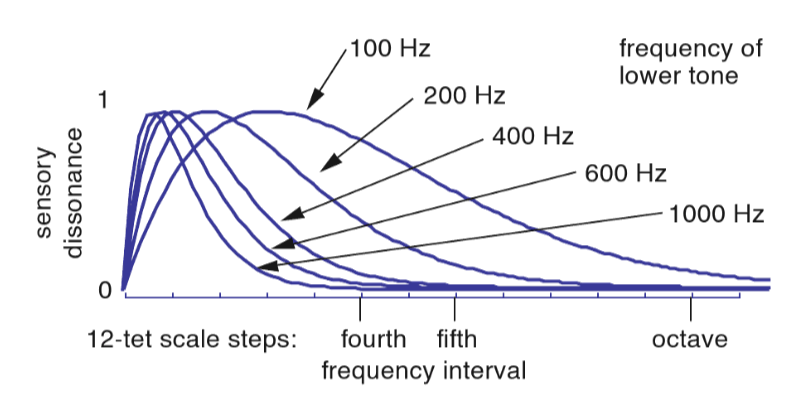
\includegraphics[width=1\linewidth]{figures/setharesTuningTimbreSpectrum2010_p47} 

}

\caption{Sensory dissonance of sine waves by interval for five frequencies. Figure \autocite[p.~47]{setharesSoundSound2005}}\label{fig:sensory-dissonance}
\end{figure}

\hypertarget{hardware-and-software-implementation}{%
\section{Hardware and Software Implementation}\label{hardware-and-software-implementation}}

\hypertarget{motion-capture}{%
\subsection{Motion Capture}\label{motion-capture}}

Motion capture data were collected using a 9 camera (8 Qualisys Miqus M3 marker and 1 Qualisys Miqus Video) system connected to a Qualisys Camera Sync Unit. Marker data were acquired at a sampling rate of 300 Hz and video data were acquired at a sampling rate of 25 Hz. Qualisys Track Manager (QTM) software version 2022.2 (build 7700) was used to collect and process the data with real-time 3D tracking data output. QTM options for `processing of every frame' and `2D data preprocessing' were disabled for real-time output to ensure minimal latency. Figure \ref{fig:exp-graph} outlines the flow of data from motion capture to sonification.

\begin{figure}

{\centering 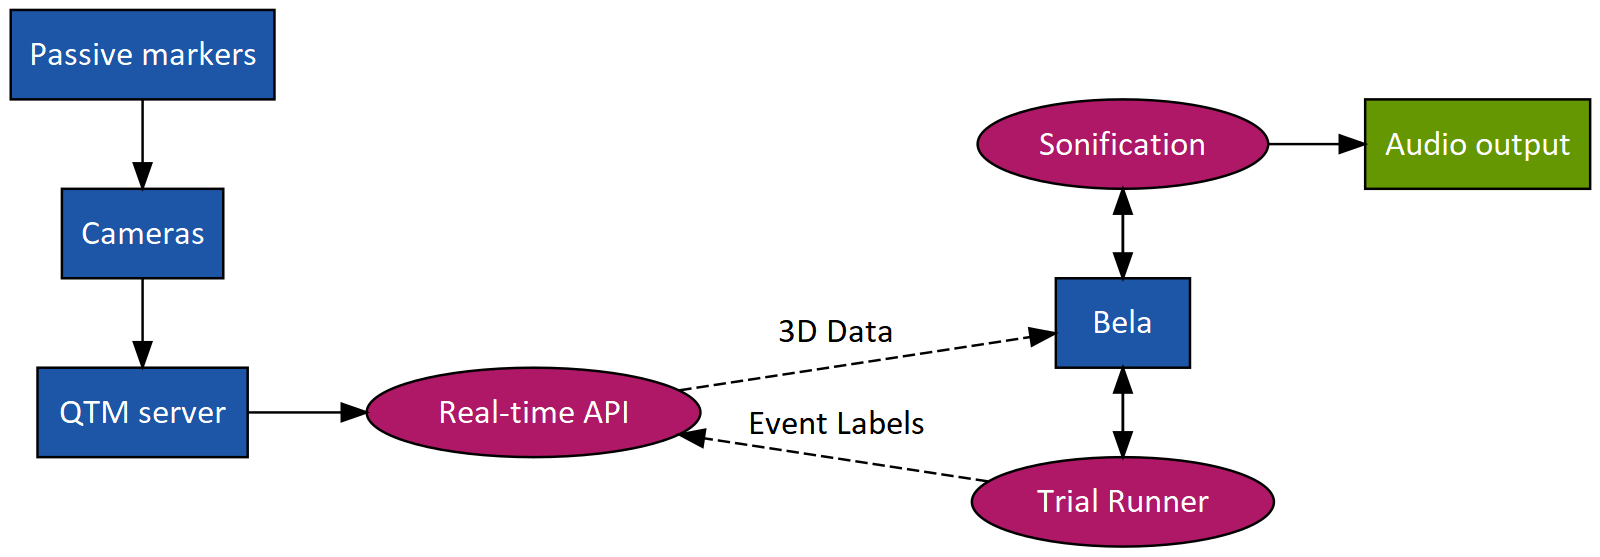
\includegraphics[width=1\linewidth]{figures/exp-graph} 

}

\caption{Low-latency sonification pipeline}\label{fig:exp-graph}
\end{figure}

\hypertarget{markers}{%
\subsubsection{Markers}\label{markers}}

For the experimental set up, one passive marker was placed on each car, and two additional passive reference markers were placed on the front corners of the track (see Figure \ref{fig:track-setup}). These additional markers provided reference points for 3D orientation of the track and the cars across trials in case of accidental track movement. QTM Automatic Identification of Marker (AIM) models were trained on variable speed sled movements along the track and were given labels for client-side identification.

\begin{figure}

{\centering 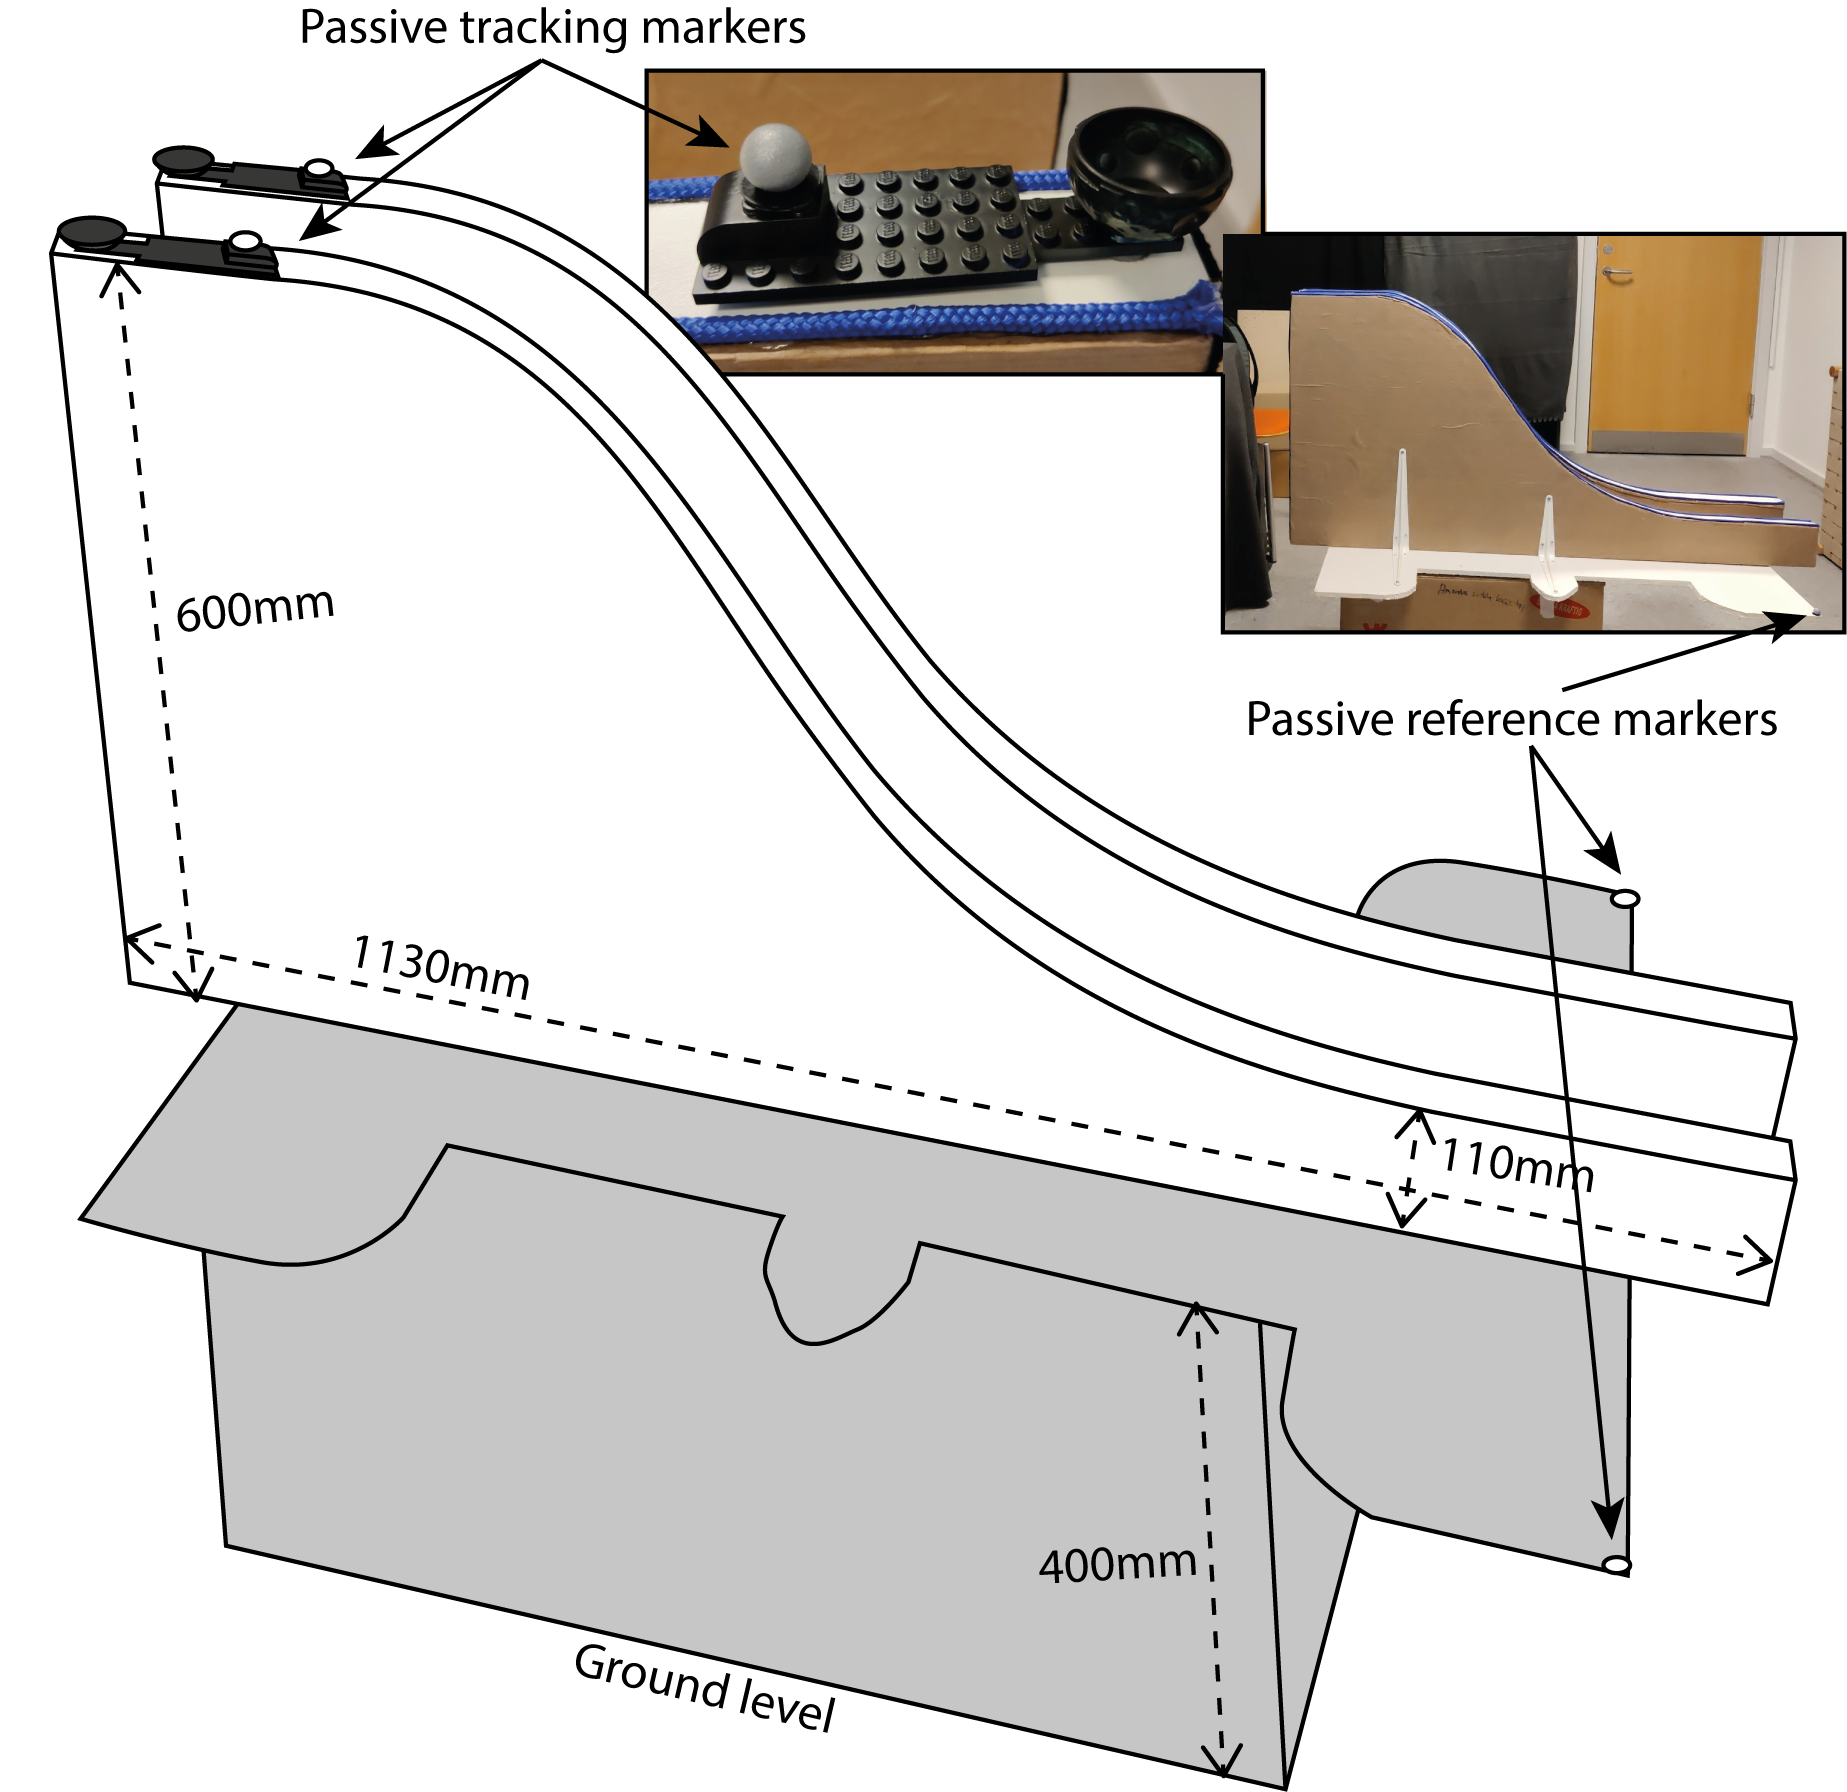
\includegraphics[width=1\linewidth]{figures/track_dimensions} 

}

\caption{Experimental track setup showing track shape and dimensions}\label{fig:track-setup}
\end{figure}

\hypertarget{sonification-1}{%
\subsection{Sonification}\label{sonification-1}}

Motion capture data were sent via UDP packets over USB networking to a Bela Mini device running version 0.3.8g running a custom C++ program\footnote{Source, data and analyses are available at \url{https://github.com/zeyus/QTM_Bela_Sonification}}. The main program loop was configured to execute every 32 samples, with an output sample rate of \ensuremath{4.41\times 10^{4}} Hz for 2 audio channels. The two audio output channels were connected to a pair of Genelec G Two active speakers. The main program used the latest available Bela platform framework \footnote{Commit ID \texttt{42bbf18c3710ed82cdf24b09ab72ac2239bf148e} from 10 August 2022: \url{https://github.com/BelaPlatform/Bela/commit/42bbf18c3710ed82cdf24b09ab72ac2239bf148e}}. The experiment flow control was automated using the defined time periods for trials and breaks between them, and paused between conditions until a button on the device was pressed to allow sufficient time for subjects to rest and answer the IOS survey.

\hypertarget{real-time-3d-data}{%
\subsubsection{Real-time 3D Data}\label{real-time-3d-data}}

A version of the Qualisys C++ SDK using protocol version 1.23 was modified to be compatible with the Bela platform and was used for communicating with QTM. To reduce latency, connection to the QTM server was made over UDP, and round-trip communication latency was verified by performing 1000 requests to the QTM server and logging the elapsed round-trip time, resulting in a mean latency of 0.25ms (SD 0.03ms, min 0.23ms, max 0.43ms).

Using the SDK, 3D streaming was initiated at the start of each sonification condition, and labelled markers were used to obtain the current position of each sled. The coordinates of the sleds were stored in a buffer containing the current and last recorded coordinates.

\hypertarget{experiment}{%
\subsection{Experiment}\label{experiment}}

\hypertarget{workflow}{%
\subsubsection{Workflow}\label{workflow}}

The experiment flow control was automated via the main C++ application running on the Bela mini. Before each experiment started, the condition order was configured in the application, and after compilation the suite of conditions and trials would run. Prior to commencement of each condition, the execution of the application halted and required manually pressing a hardware button on the Bela to continue, this was to allow sufficient time for subjects to rest and to answer the IOS survey between conditions. After commencement of a condition, all trials for that condition were run consecutively with 15 second breaks between them. Three tones played immediately prior to each trial to indicate the start of the trial, and a single tone played at the end of the trial to indicate the start of the break and participants would move their sleds to the start of the track.

\hypertarget{event-labels}{%
\subsubsection{Event Labels}\label{event-labels}}

From the main Bela application, event labels indicating the start of an experiment suite, start and end of a condition and the start and end of individual trials were sent to the QTM server. These labels appear in the recorded 3D data and were exported alongside the marker positions for use in analysis and enable data to be segmented into their respective conditions and trials.

\hypertarget{task-and-procedure}{%
\section{Task and Procedure}\label{task-and-procedure}}

Participants were asked to sit on opposite sides of the track structure and familiarize themselves with the movement of the sleds along the tracks. They were instructed to continuously move the sleds along the track from end to end, as rapidly as possible while remaining spatially synchronized with their partner's position on their respective track, using sounds they may hear during the various conditions to assist them. After the conclusion of subject briefing and they had indicated they were ready, they were blindfolded for the duration of all trials within a condition, with a pause between conditions where they could rest and remove the blindfold.

(prioritized comfort, allowed choice of arm despite handedness) {[}why this many, why not more, etc, ethics{]} Subjects were given and signed an informed consent form {[}appendix\ldots{]} and information sheet {[}appendix\ldots{]}\ldots{} and were under the umbrella project\ldots{}

\hypertarget{sonification-strategy-conditions}{%
\subsection{Sonification Strategy Conditions}\label{sonification-strategy-conditions}}

The experiment consisted of three conditions that vary the sonification strategy employed, namely: a no sonification control condition, a task-oriented sonification strategy and a synchronization-oriented sonification strategy. Each condition consisted of one practice trial of 30 seconds duration, and three main trials of 90 seconds each. Before each practice trial, subjects were reminded that it was a shorter trial and that they may use it to experiment with the sonification.

\hypertarget{no-sonification}{%
\subsubsection{No sonification}\label{no-sonification}}

In the no sonification condition, only the motion capture data from participants' sleds were recorded, and subjects could use the audible sounds of the sleds moving along the track to align themselves with their partner.

\hypertarget{task-oriented-sonification-strategy}{%
\subsubsection{Task-oriented sonification strategy}\label{task-oriented-sonification-strategy}}

Task oriented sonification represented the position of each sled along the length of the track as a synthesized tone that varied in frequency from highest to lowest at the start and end of the track respectively. One sled produced a higher frequency overtone, while the other produced a lower frequency undertone. If subjects were at the exact same x-coordinate, the two tones would be a perfect fifth apart, creating a harmonious chord, as the sleds drift further apart, the frequency difference would deviate from the perfect fifth and create a more discordant sound, Figure \ref{fig:task-illustration} illustrates the implementation of the task-oriented sonification strategy. This strategy was selected for sonifying the movement along the track, i.e.~the task required of subjects .

\begin{figure}

{\centering 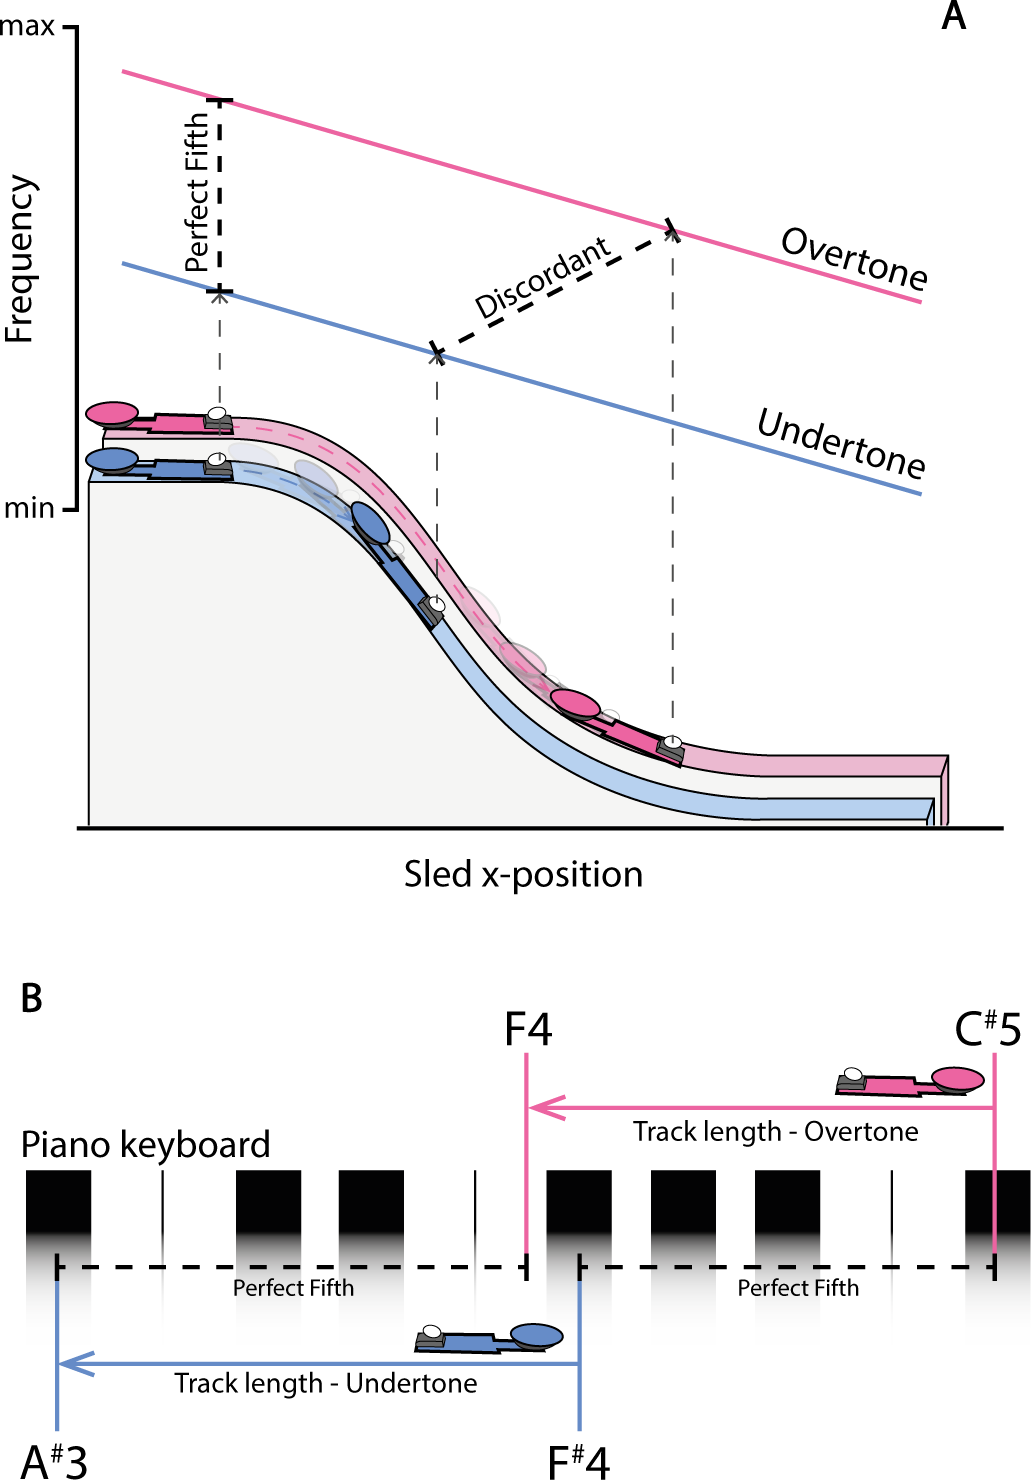
\includegraphics[width=1\linewidth]{figures/task_sonif_illustration} 

}

\caption{Task}\label{fig:task-illustration}
\end{figure}

\hypertarget{synchronization-oriented-sonification-strategy}{%
\subsubsection{Synchronization-oriented sonification strategy}\label{synchronization-oriented-sonification-strategy}}

The sonification strategy oriented around synchronization represented the position of the sleds relative to each other, where subjects with sleds at the same x-coordinates would hear a harmonious perfect fifth chord. When sleds would drift apart, the overtone amplitude would decrease, and the undertone frequency would change based on the distance between the two sleds, Figure \ref{fig:sync-illustration} illustrates the implementation of the synchronization-oriented sonification strategy.

\begin{figure}

{\centering 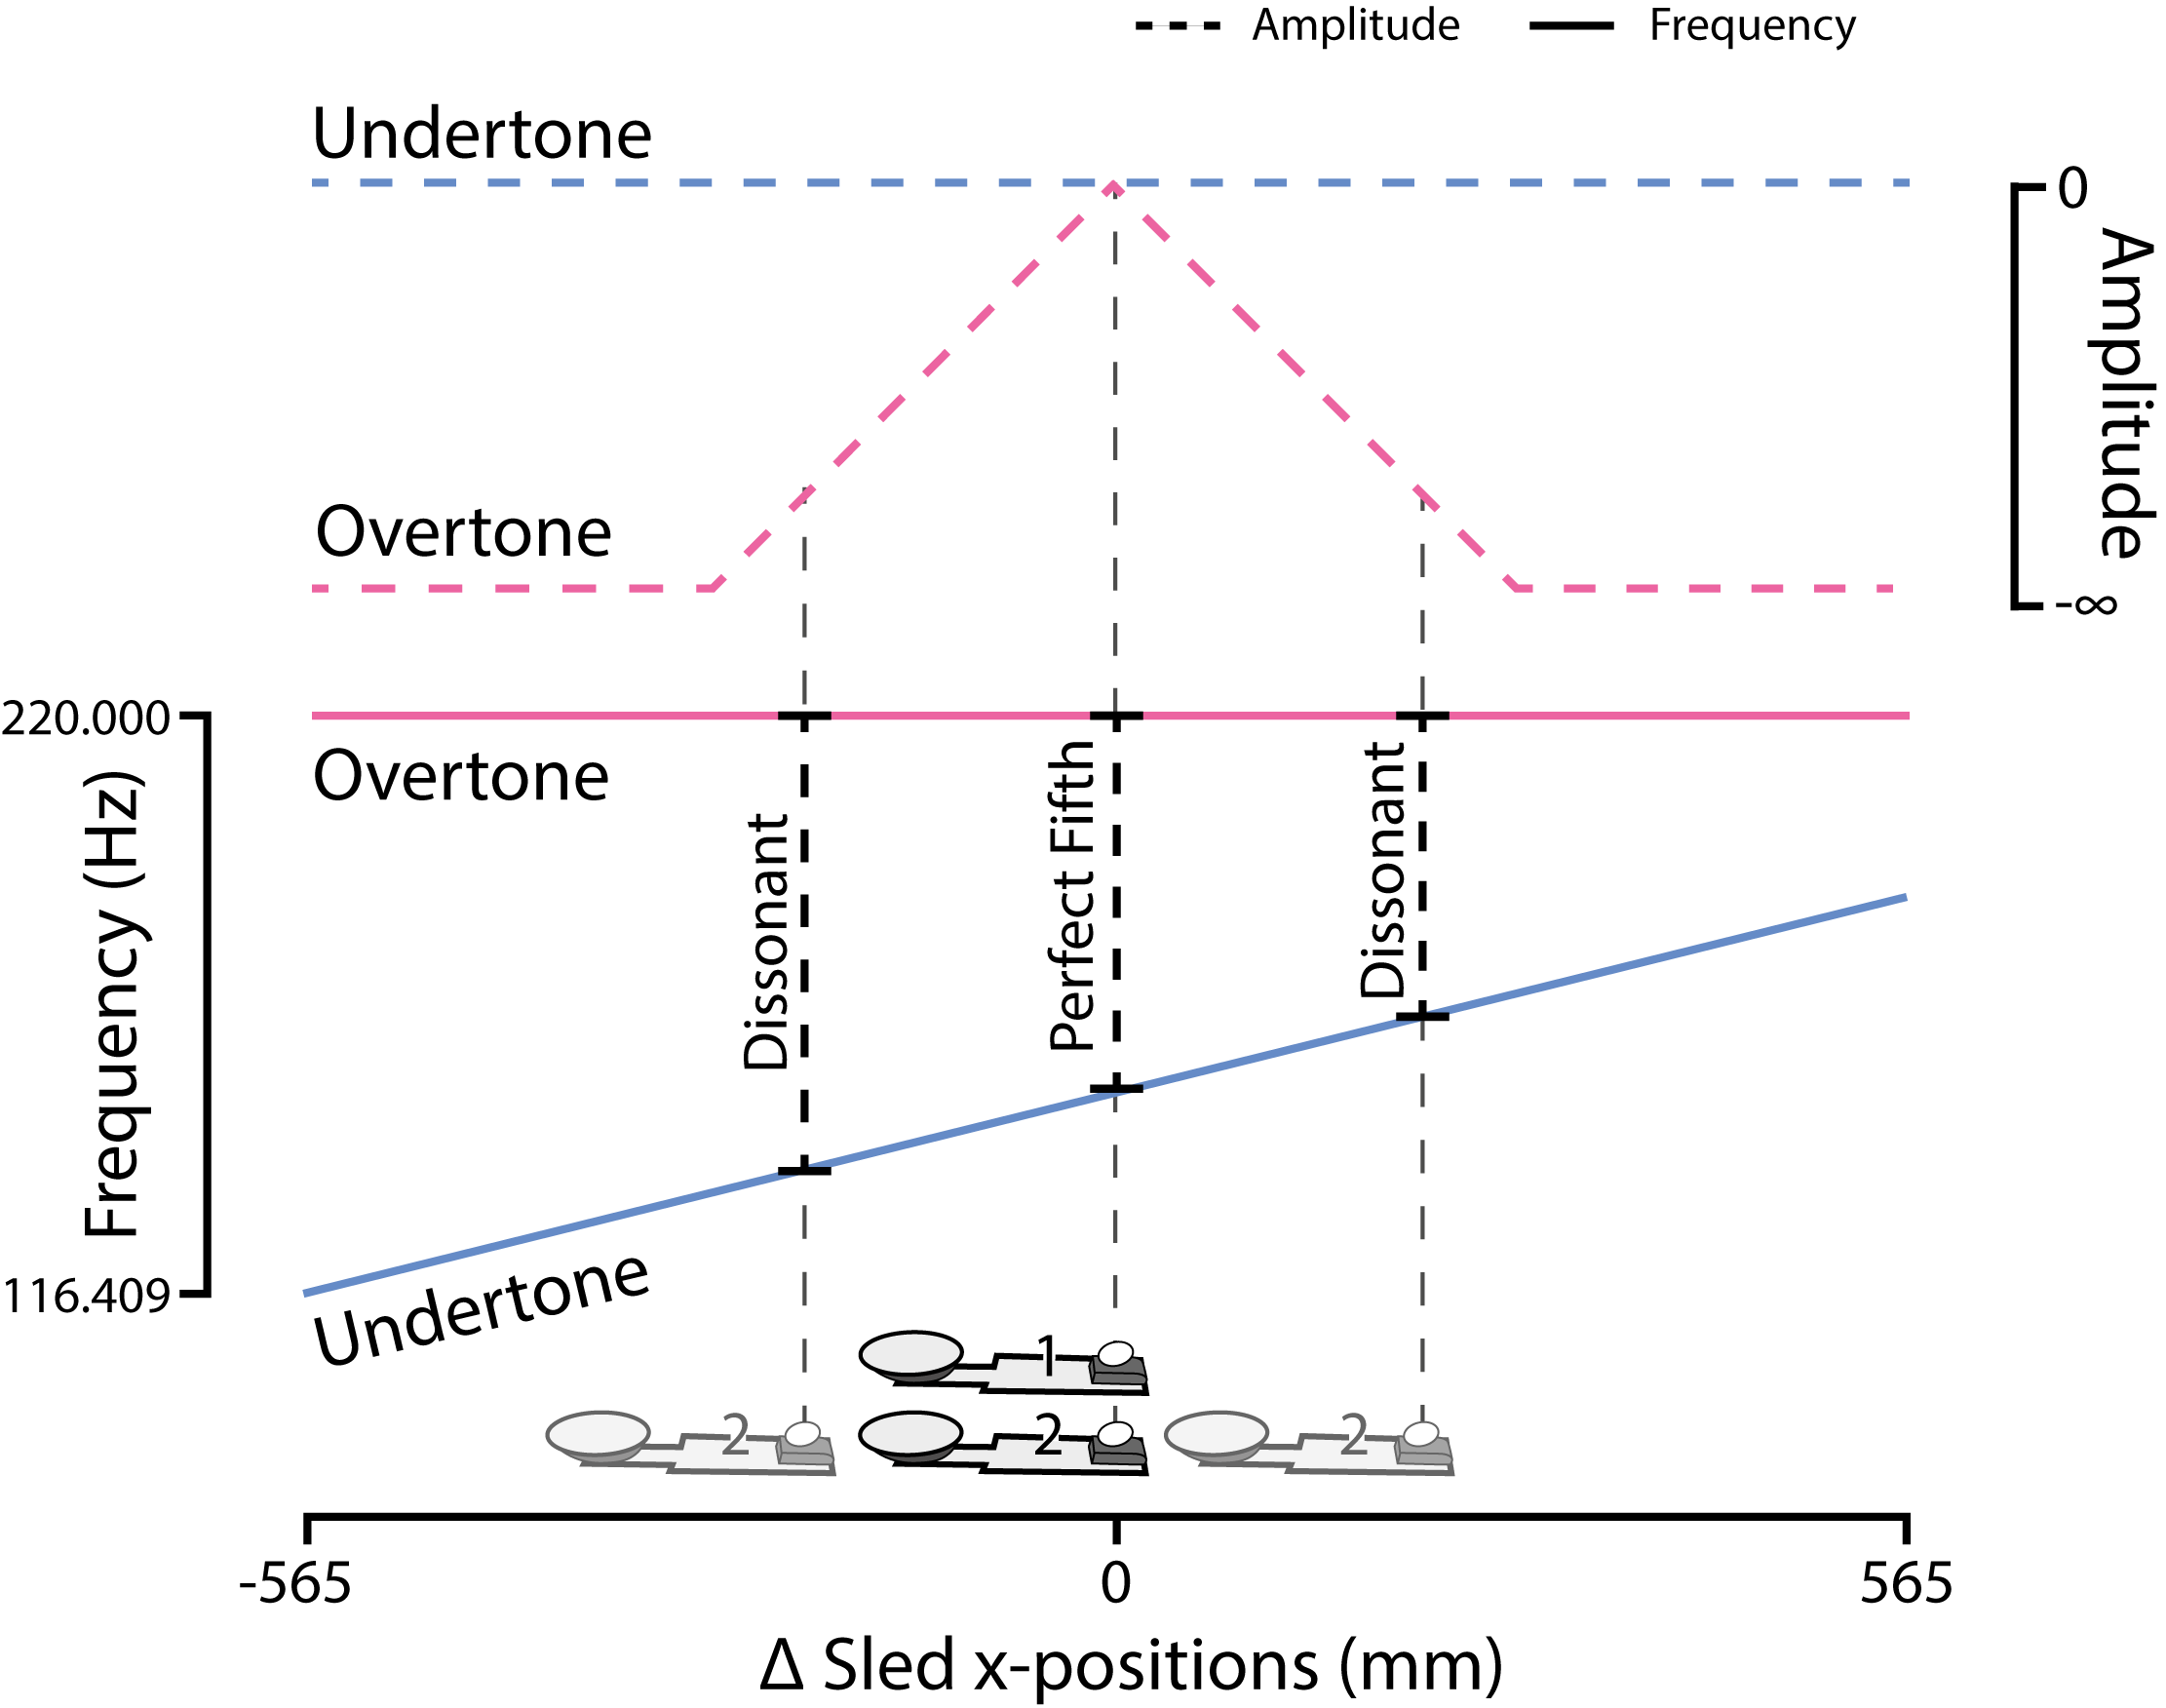
\includegraphics[width=1\linewidth]{figures/sync_sonif_illustration} 

}

\caption{Sync}\label{fig:sync-illustration}
\end{figure}

\hypertarget{analyses}{%
\section{Analyses}\label{analyses}}

General timing stuff, project specific stuff.

\hypertarget{data-preprocessing}{%
\subsection{Data Preprocessing}\label{data-preprocessing}}

\hypertarget{qtm}{%
\subsubsection{QTM}\label{qtm}}

Each session recorded had the AIM model applied to the duration of the recording, and labelled markers were manually verified and adjusted as required to ensure that for each completed trial, there was 100\% coverage of the marker data.

\hypertarget{d-data}{%
\subsubsection{3D Data}\label{d-data}}

3D data were exported from QTM and several preprocessing scripts were developed using the R programming language. Data were imported and collated by unique subject pair, condition and trial using the indices of the associated event labels, subsequently, practice trials, data outside of trials and invalid trials were removed. Invalid trials were defined as trials that did not have both a start and end event label. Trajectories were then created from marker x-coordinate time series using the R package \texttt{mousetrap} \autocite{mousetrap2021} which was designed to aid analyses of mouse movement trajectories, and is able to be applied to arbitrary spatial data. The starting position of trajectories were aligned to account for track movement between trials, and x-axis trajectories were standardized within trials to have a mean of 0 and a range from -1 to 1 allowing comparison between subject pairs, conditions and trials. Visual inspection of trajectory data was performed, and six trials where participants had lost control of the sleds were truncated to the time of the incident. This left a total of 44 experimental trial observations (38 complete and 6 truncated), meaning data were available for all subject pairs in all conditions, with one single trial excluded from one subject pair.

\hypertarget{subject-synchronization}{%
\subsection{Subject Synchronization}\label{subject-synchronization}}

\hypertarget{distance}{%
\subsubsection{Distance}\label{distance}}

Distance between subject sleds is a useful proxy for determining the level of success of synchronization, where a trial where subjects move perfectly together would result in a delta of zero for each time point, and large distances would indicate that they were unable to synchronize their sled movements. Absolute distance deltas between the standardized x-coordinates of subject pairs were calculated for each time point by trial and condition. Mean deltas per condition were calculated per subject pair, resulting in\ldots.. (Figure \ref{fig:pairwise-position-delta})
Table\ldots{}

\begin{figure}

{\centering 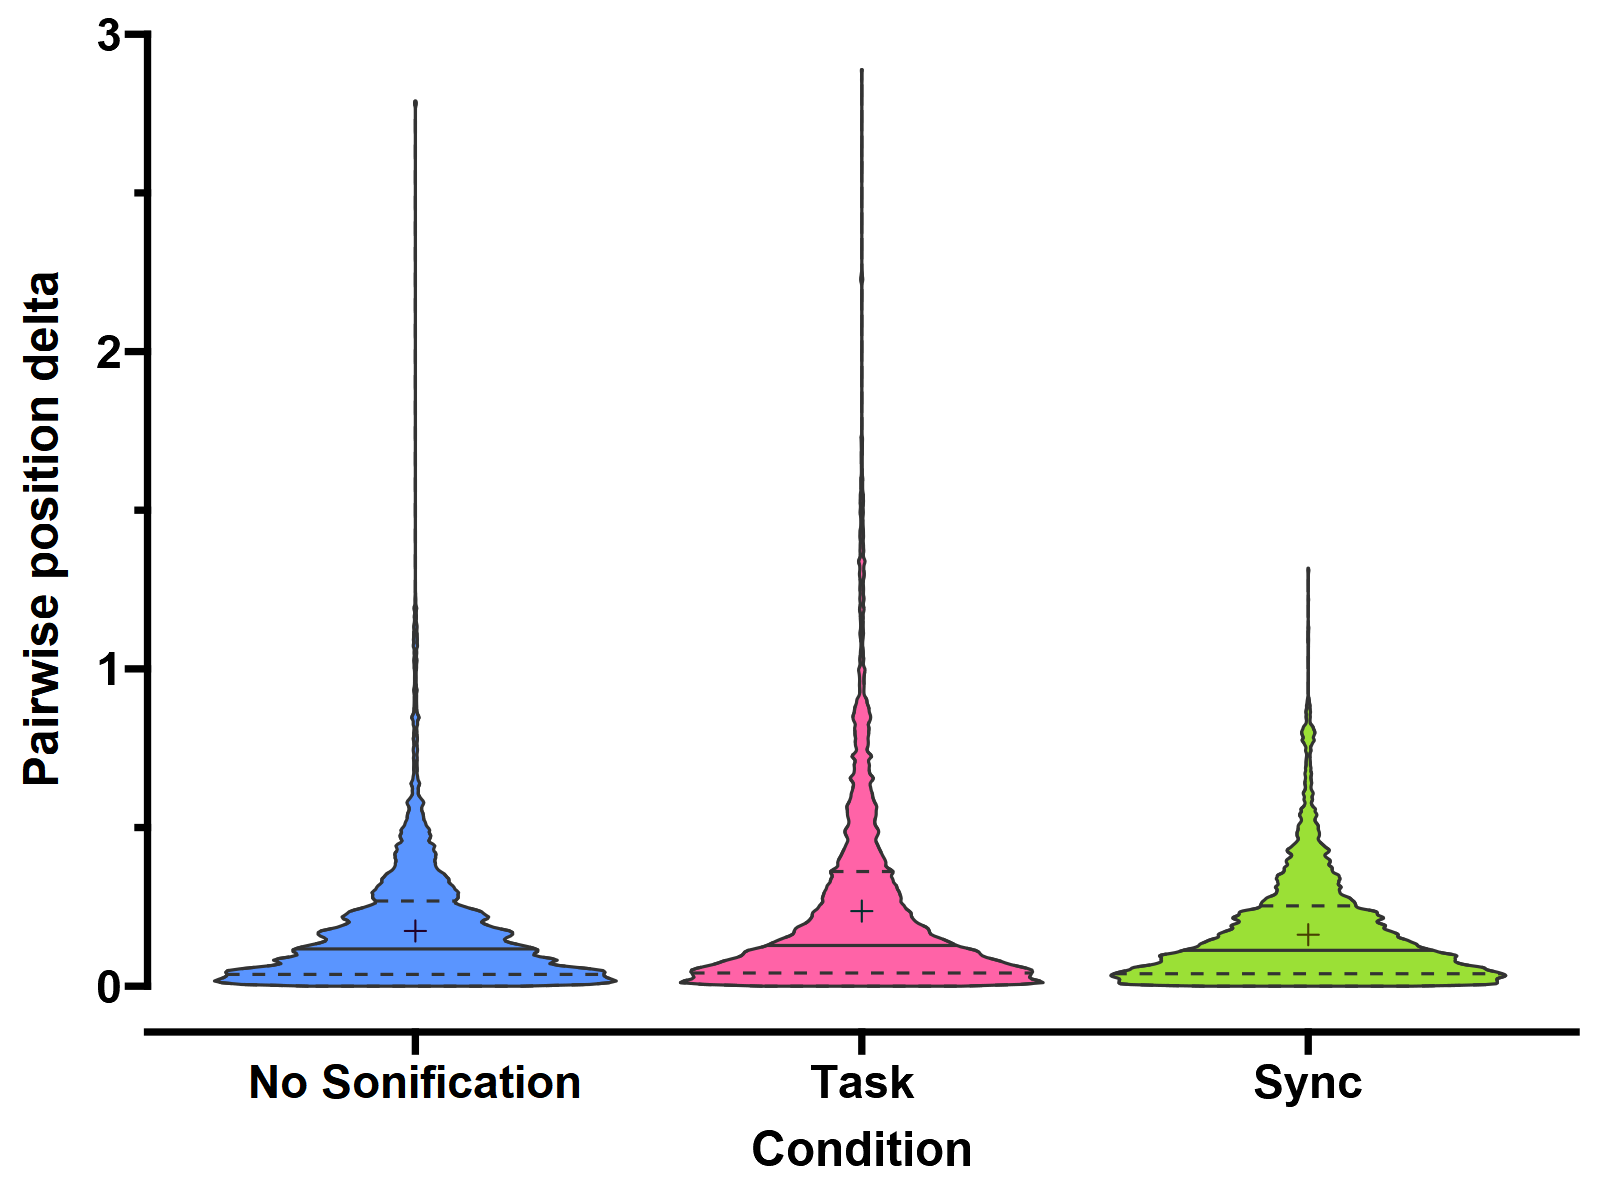
\includegraphics[width=1\linewidth]{figures/parwise_position_delta} 

}

\caption{Plot of pairwise position delta for each subject pair}\label{fig:pairwise-position-delta}
\end{figure}

\hypertarget{instantaneous-phase-angle-of-trajectories}{%
\subsubsection{Instantaneous Phase Angle of Trajectories}\label{instantaneous-phase-angle-of-trajectories}}

Hilbert transform\ldots etc.etc, distance doesn't tell the whole story\ldots.what if some move really slow, fast, etc\ldots.esentially a waveform / signal data\ldots.(Figure \ref{fig:mean-instantaneous-phase-angle-circular-plot})

The results showed that the mean angle difference
was 8.861° ± 0.067° (SD) for the no sonification condition,
14.211° ± 0.216° (SD) for the task condition, and
8.749° ± 0.075° (SD) for the sync condition. (Figure \ref{fig:mean-instantaneous-phase-angle-circular-plot}).

\begin{figure}

{\centering 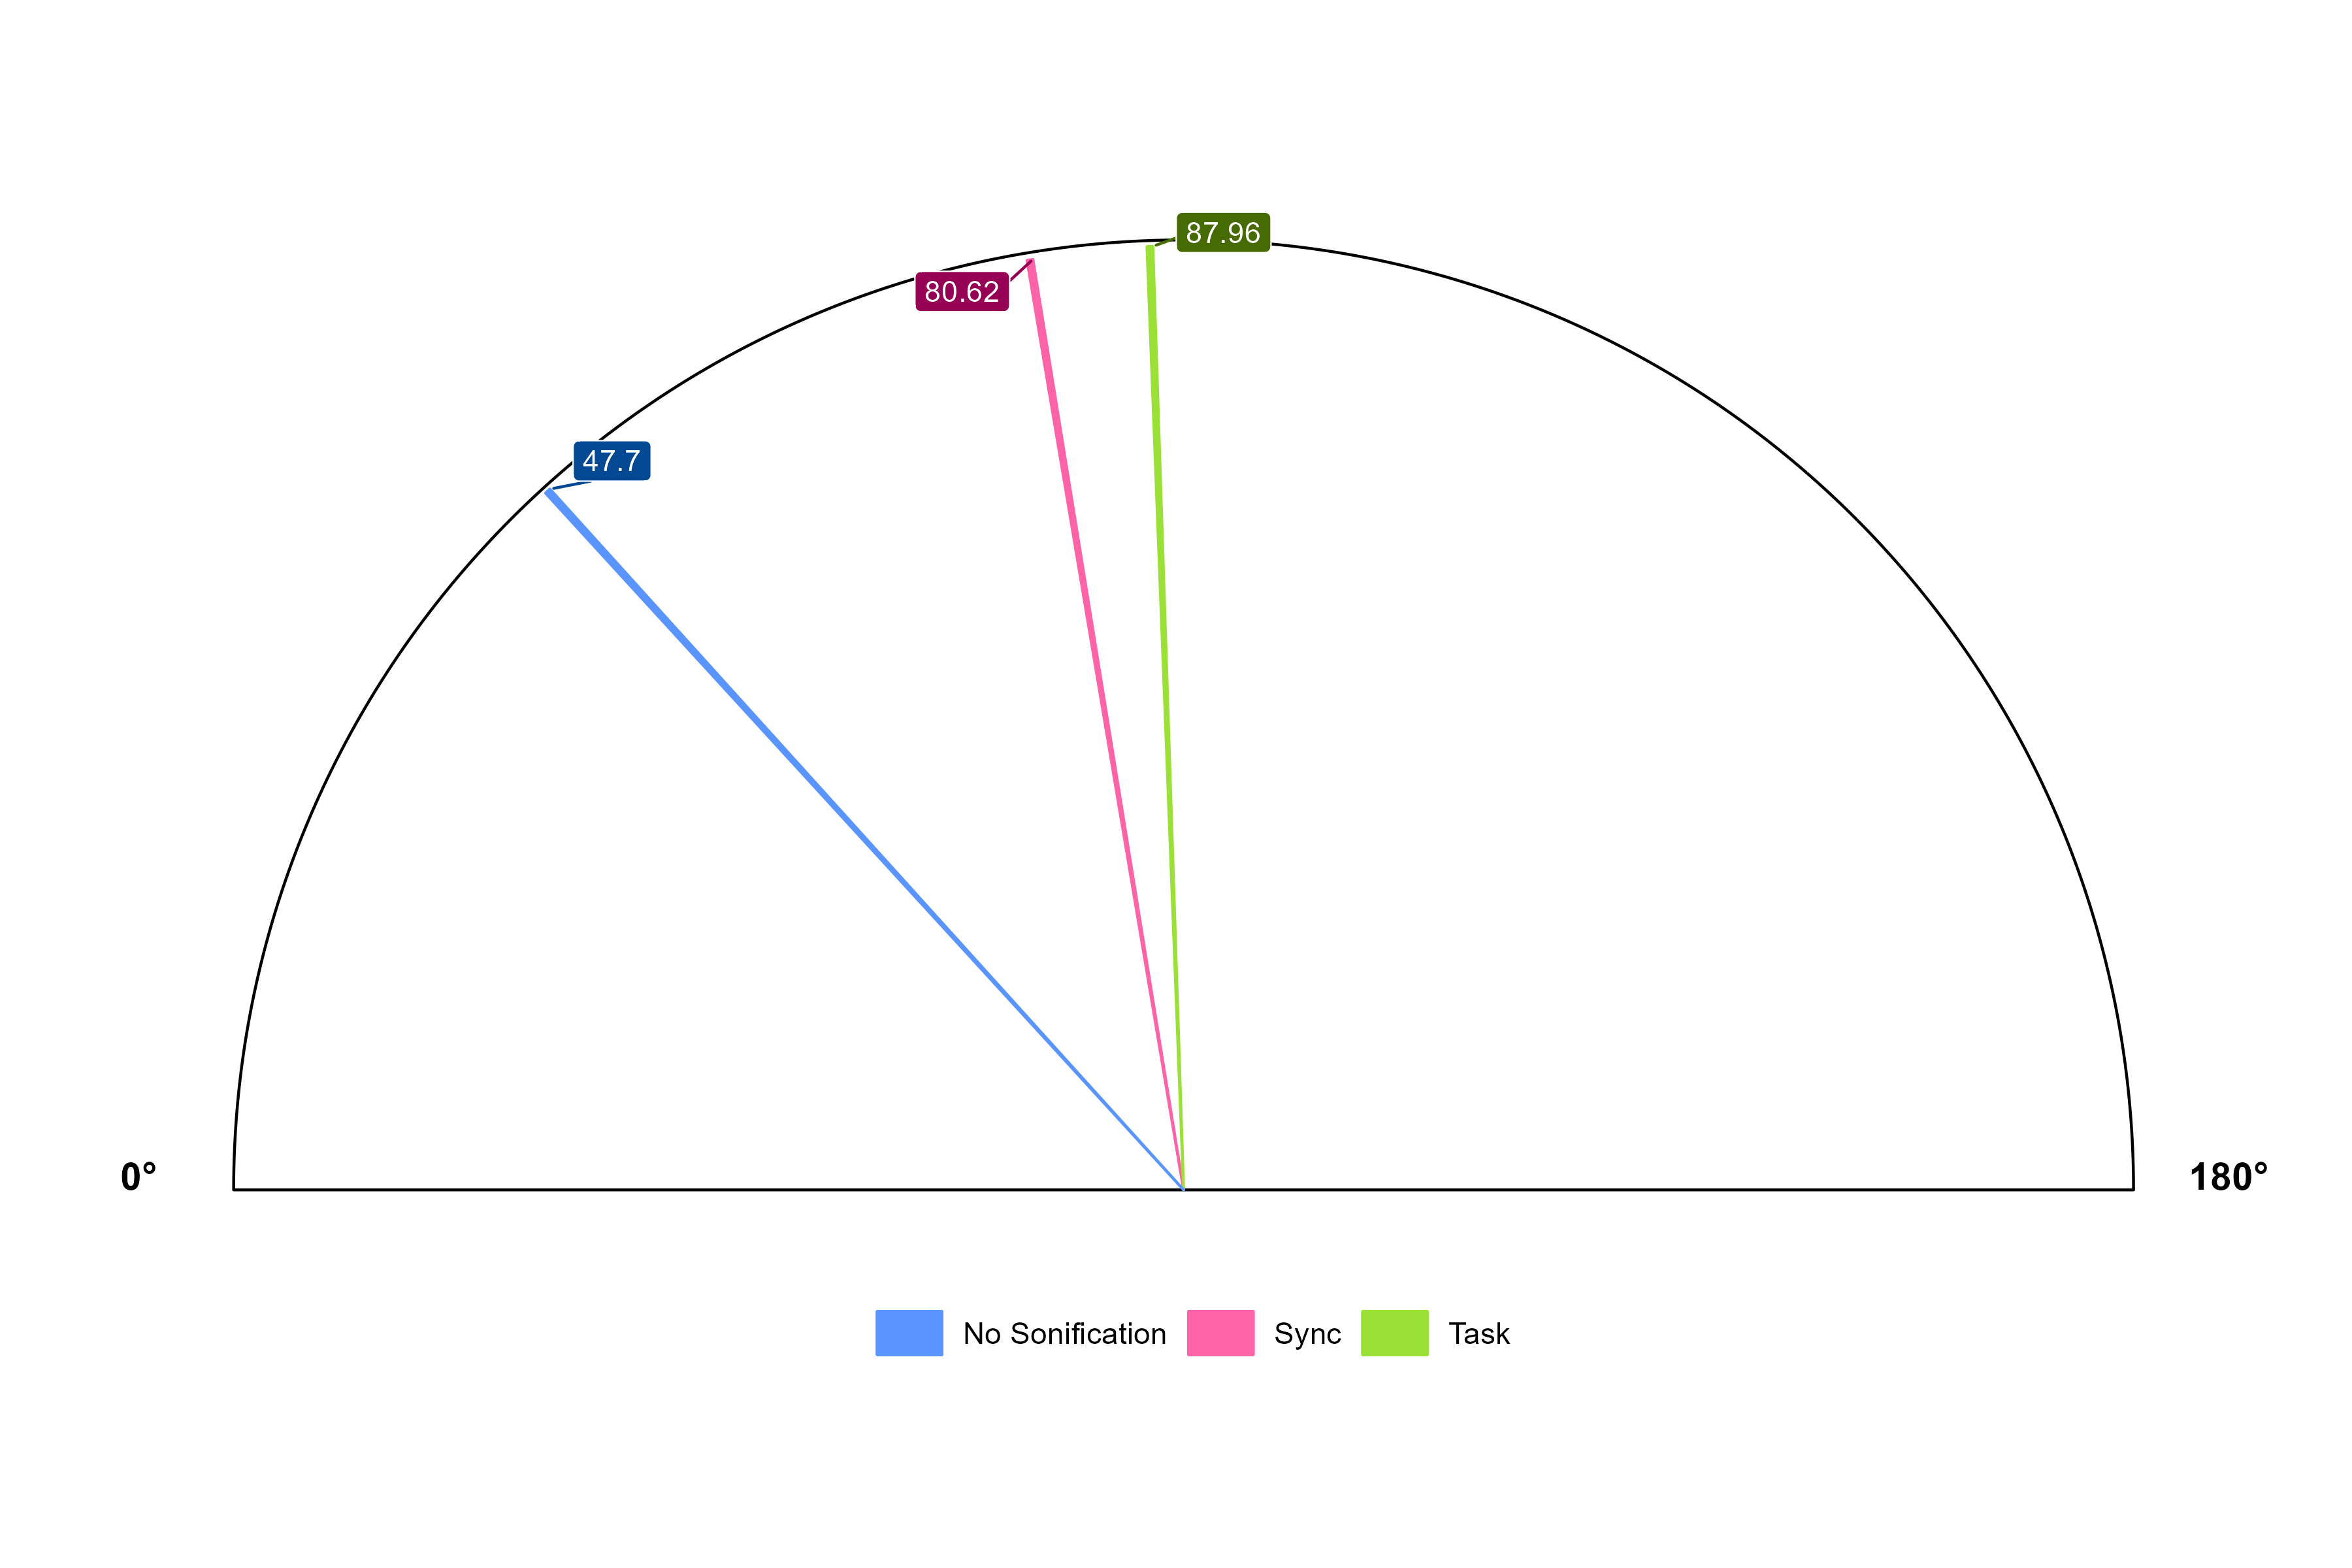
\includegraphics[width=1\linewidth]{figures/mean_condition_phase_angles_mean_sd} 

}

\caption{Plot of mean absolute instantaneous phase angles of experimental conditions with the length of the needles representing the standard deviation as a percentage of 90 degrees. No Sonification condition mean phase angle =  8.861 (sd =  0.067 ) degrees, task sonification condition mean phase angle =  14.211 (sd =  0.216 ) degrees, sync sonification condition mean phase angle =  8.749 (sd =  0.075 ) degrees.}\label{fig:mean-instantaneous-phase-angle-circular-plot}
\end{figure}

\hypertarget{dynamic-time-warping}{%
\subsection{Dynamic Time Warping}\label{dynamic-time-warping}}

\begin{figure}

{\centering 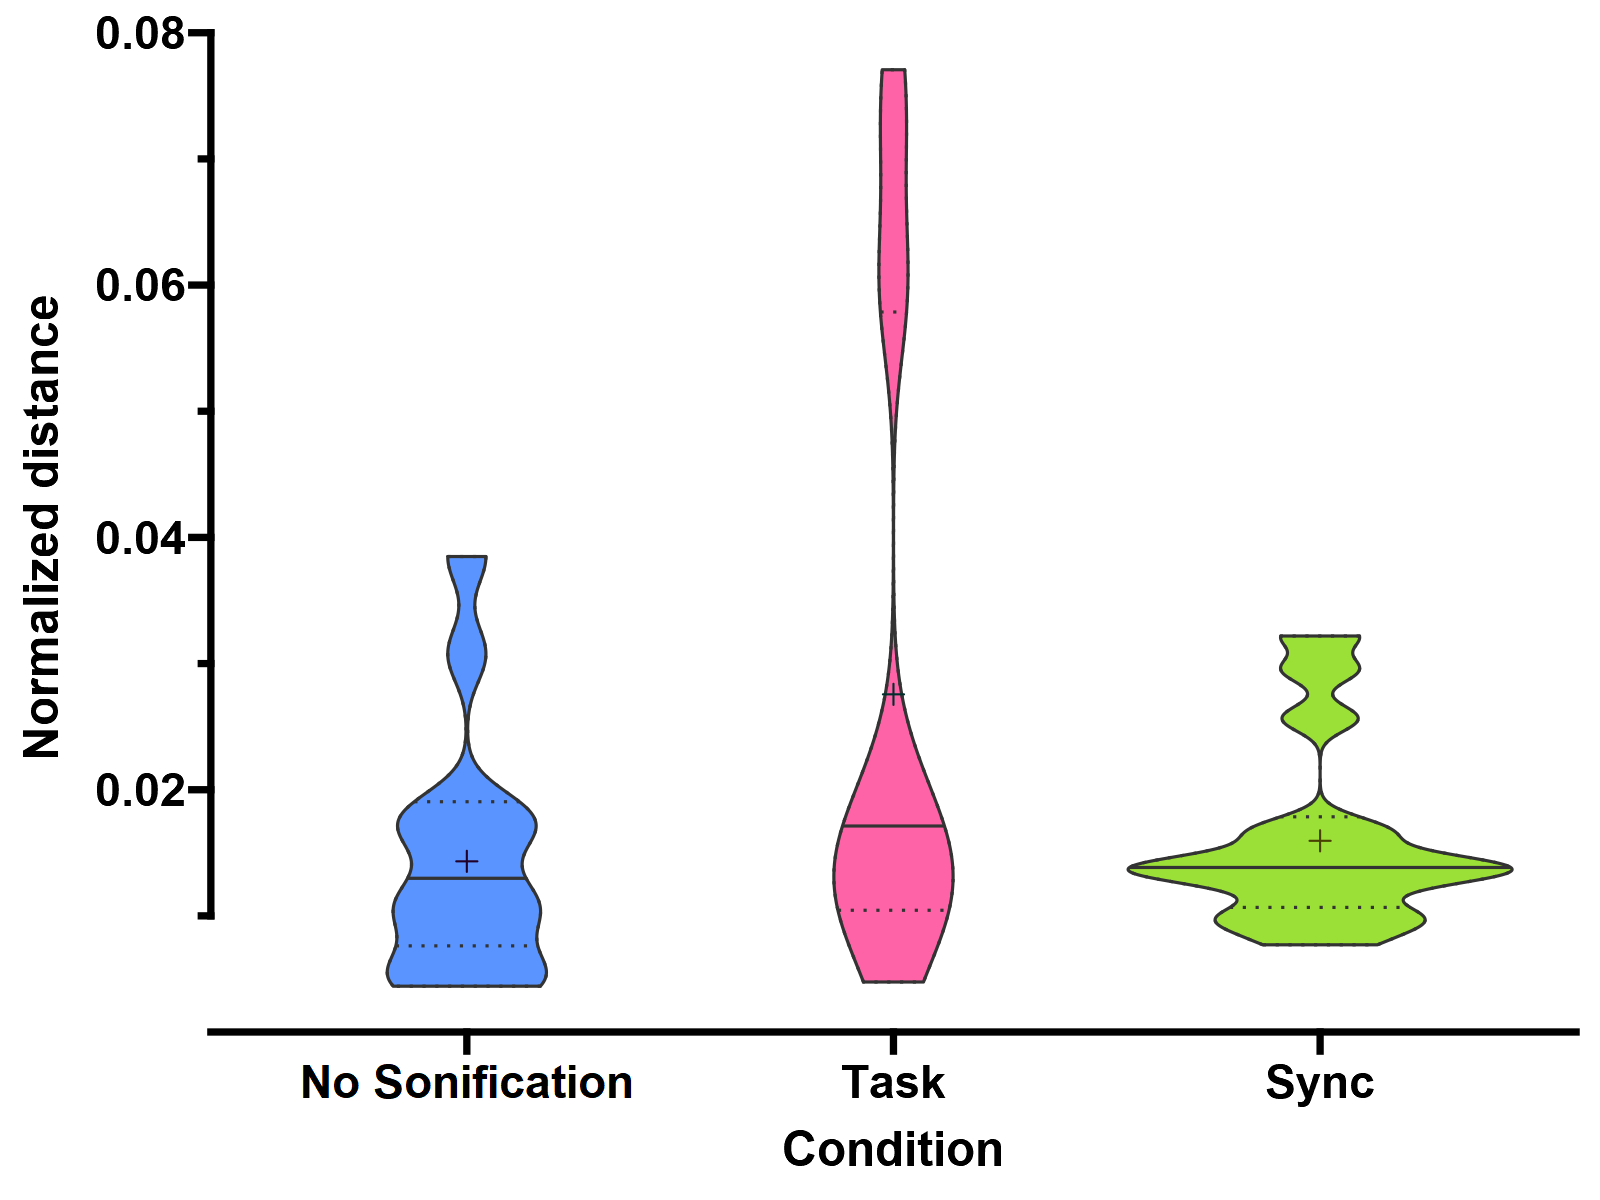
\includegraphics[width=1\linewidth]{figures/dtw_summary} 

}

\caption{Distribution density plot of normalized dynamic time warp path distance between paired trajectories by condition. The mean normalized distance is shown as a point (+), the 20th and 80th percentiles are shown as dashed lines and the 50th percentile is shown as a solid line. No Sonification condition normalized distance mean  =  0.014 (sd =  0.01 ) degrees, task sonification condition normalized distance mean =  0.028 (sd =  0.025 ) degrees, sync sonification condition normalized distance mean =  0.016 (sd =  0.007 ) degrees.}(\#fig:dtw-plot, )
\end{figure}

\hypertarget{learning}{%
\subsection{Learning}\label{learning}}

{[}optional{]} include simple analysis of mean / sd by trial

\hypertarget{results}{%
\section{Results}\label{results}}

\hypertarget{testing-different-model-outputs-tables}{%
\subsubsection{Testing different model / outputs / tables}\label{testing-different-model-outputs-tables}}

\hypertarget{synchronization}{%
\subsection{Synchronization}\label{synchronization}}

\hypertarget{distance-1}{%
\subsubsection{Distance}\label{distance-1}}

\hypertarget{angle}{%
\subsubsection{Angle}\label{angle}}

\hypertarget{discussion}{%
\section{Discussion}\label{discussion}}

{[}Explain{]}

How might our task be affected by musical training? ``Successful music performance requires that musicians monitor the auditory consequences of their actions. Years of training on an instrument lead to strong associations between a given movement or set of movements and a given auditory outcome.'' (Loehr et al., 2013)
ML model applications in this project?

Mention the marker placement as being problematic. Also the number of reference markers\ldots also that we wanted to use headphones\ldots{}
Mention analysis of learning effect, not enough data here, too many invalid trials, but would be interesting to see if participants ``learn'' the sonification schemes

• How does our task compare to e.g.~Loehr et al.~piano duet task?
• What can and can't our task reveal?
o Can't say that only one of the participants makes a mistake, since the goal is to in sync with each other, without a general ``tempo'' to follow
• Individual representations vs joint outcome representations?
o Often can't mirror the other person exactly

if someone wanted to reproduce we can talk about things like the height of the track, the width of the base making it less comfortable, the range in participant music experience, also the fact that the mocap lab is small and there were problems making camera trakcing more difficult.

and of course all the stuff about different sonification options and testing ranges of values to see what works, and whole new strategies we haven't thought of using headphones to stop the track noise which subjects noted they used\ldots{}

and of course we can talk about that in relation to the results, lack of results, why we might be seeing the data we see,
and especially that we actually managed to create a low-latency method for sonification of /arbitrary/ data, and we used it for an expensive mocap setup but this could be applied to outputs from machine learning models (i.e.~webcam object tracking) or even other low-cost hardware like wiimotes or something

\begin{figure}

{\centering 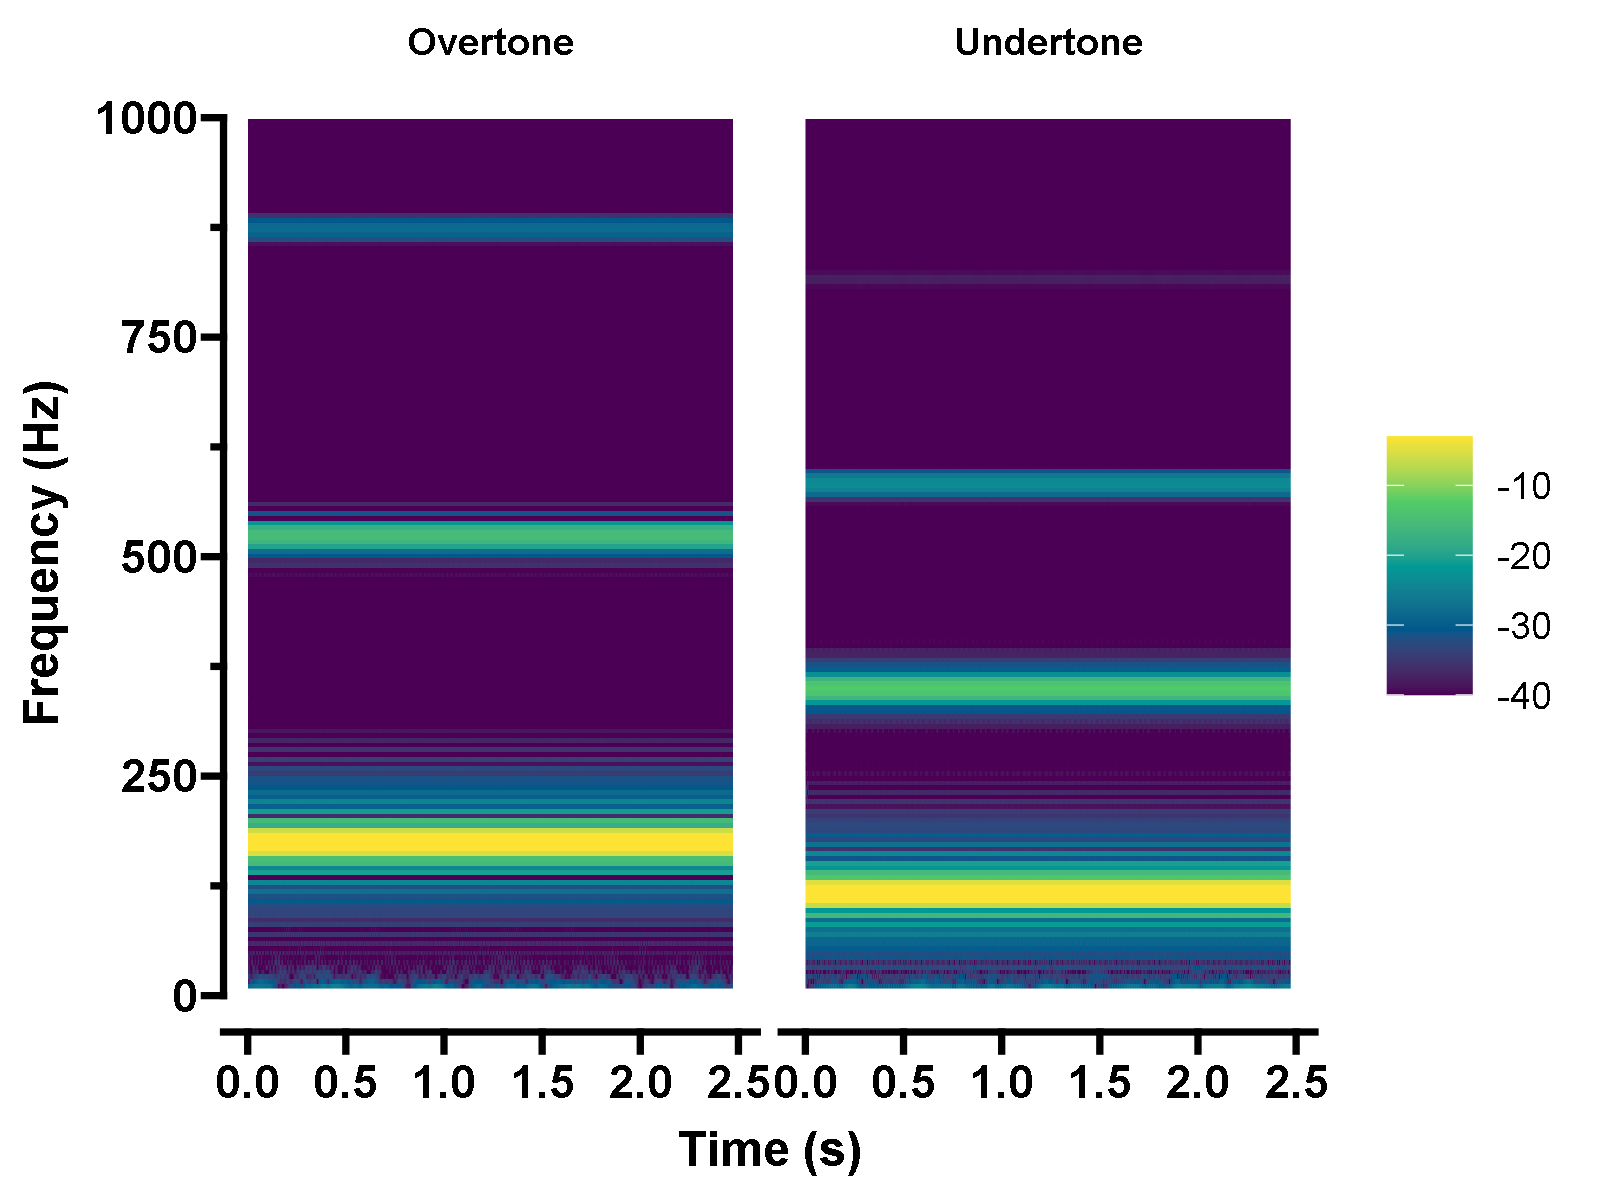
\includegraphics[width=1\linewidth]{figures/spec_tones} 

}

\caption{Spectral analysis of the two base frequency audio files}\label{fig:stimuli-spectra}
\end{figure}
\balance
\clearpage


\printbibliography[title=References,heading=bibintoc]

\end{document}
